\chapter{Learning Off-label Drug Usages}

\section{Introduction}
Off-label drug use occurs when a drug is used in a manner that differs
from its approved use as described by its FDA label.  This practice is
common and provides a pathway for clinical innovation.  However, such
uses escape the scientific scrutiny that goes into the labeling and
marketing of new medicines \cite{Stafford2012,Pan2012}.  Estimates
from office-based practices found that 21\% of prescriptions are
off-label .  Of these, 73\% had little or no scientific support
\cite{Radley2006,Chen2009}, raising concerns about patient safety and
costs to the healthcare system.  For instance, tiagabine was approved
for use as an adjunctive therapy for partial epilepsies.  However,
when used as the sole or primary treatment, it was found to cause
seizures.  In 1998, 20\% of uses of tiagabine were off-label, but by
2004 this fraction had increased to 94\% \cite{Flowers2006}.

Off-label use is to some extent inevitable because not every condition
can be tested during pre-approval \cite{Kimland2012,Epstein2012}.
Nevertheless, all stakeholders in the health care system have an
interest in the timely, systematic detection of off-label use.  Drug
manufacturers are required to report on off-label use observed in
post-marketing surveillance in the European Union \cite{Morris2012}.
Regulatory agencies and clinical researchers can use knowledge of
emerging off-label uses to identify potential benefits or risks that
require further investigation.  Furthermore, patients and their health
care providers should minimize exposure to risks without clinical
benefit.  Unfortunately, current pharmacovigilance and post-market
surveillance efforts in the United States do not monitor off-label
use.  Standard surveillance approaches using the FDA's Adverse Event
Reporting System (FAERS) do not specifically account for use in
off-label indications; efforts such as the Observational Medical
Outcomes Partnership (OMOP) and the Mini-Sentinel projects do not
specifically look at off-label use \cite{Platt2012}; and physician
surveys, such as the NDTI, are limited by coverage, timeliness and
cost.

In this work, we focus on the problem of automatically discovering
off-label uses of drugs—defined as the use of drugs for unapproved
indications—from electronic health records and rank the newly
discovered uses for follow up based on risk and cost metrics.  At its
core, we need to match drugs to the diseases they are being used to
treat.  We refer to such matches as drug-indication usage pairs, and
say that a used-to-treat relationship exists between the drug and
disease (the indication).

Previous work by Wei et al \cite{WeiQi2013} used structured and
semi-structured data from RxNorm, MedlinePlus, SIDER 2, and Wikipedia
to compile a comprehensive list of drug-indication usage pairs.
Similarly, Xu et al \cite{Xu2013} used data from ClinicalTrials.gov
and Medline to compile such a list.  However, both these efforts rely
on curated data sources that may not reflect current clinical
practice.  In contrast, the data in electronic health records
represents current clinical practice and can discover such usages
before they are incorporated into curated data sources.

Thus, widespread adoption of electronic medical records (EMR) provides
an opportunity to detect off-label use in an automated, scalable and
timely manner \cite{Morris2012}.  However, structured data in EMRs
usually do not explicitly link diseases to the drugs being used to
treat them \cite{Pan2012} and is not as comprehensive as the free text
of clinical notes \cite{Poissant2010}.  Therefore, Natural Language
Processing (NLP) is often used to extract used-to-treat relationships
between drugs and indications from clinical text.  Previous efforts
use one of two approaches: the first approach identifies used-to-treat
relationships at the level of specific occurrences of drugs and
indications in text.  For example, from the phrase, “on Plavix for
PAD”, a used-to-treat relationship between clopidogrel and peripheral
artery disease is detected.  Submissions to the 2010 i2b2 NLP
Challenge \cite{Uzuner2011} represent the state of the art of this
approach.  The best performing methods require examples of text in
which occurrences of drugs, indications and the relationships between
them are explicitly labeled \cite{Chapman2011}. Such labeled training
data is difficult to obtain (the i2b2 Challenge included 871 labeled
notes) and collections of labeled text covering all drugs and
indications are not available. To overcome this limitation, an
alternative approach is to infer used-to-treat relationships at the
population level—rather than asking whether a sentence or note implies
an instance of a used-to-treat relationship, we ask whether the data
as a whole suggests that a used-to-treat relationship holds in general
\cite{Chen2008,Rindflesch2005,Lependu2012}.  The basic idea is to
count the number of times a drug and indication are mentioned in the
same clinical record, and compare that count to the expected
co-mentions by chance.  We have previously used such an approach for
detecting drug-related adverse events \cite{Lependu2013}, identifying
drug-drug interactions \cite{Iyer2013}, and profiling drug usages
\cite{Lependu2012}.  Such approaches can use relatively simple,
methods for detecting drug and indication mentions in free text that
do not require labeled text corpora for training.  As a result, such
approaches scale to very large collections of clinical text and the
entire range of drugs and indications encountered in the data.  In
Jung et al \cite{Jung2013}, we demonstrated that it is possible to
detect off-label usage using inputs derived from clinical text,
combined with prior knowledge of drugs and indications from Medi-Span
and DrugBank.  Other researchers \cite{Li2011} have also used prior
knowledge of known usages to match drugs and known indication mentions
in clinical notes demonstrating that use of prior knowledge does
improve the accuracy of detecting used-to-treat relationships.

In this paper, we build on our previous work. First, we have improved
the accuracy of the classifier by taking known usage into account when
counting co-mentions of drugs and indications in the clinical notes in
order to reduce spurious associations arising from co-morbidities.
Second, we have filtered the set of predicted novel off-label usages
for support in independent, complementary data sources.  We also
filtered out spurious associations due to causal relationships using
the SIDER 2 database \cite{Kuhn2010}.  Finally, in order to triage the
off-label uses for follow-up, we developed indices of drug cost and
risk associated with a drug’s usage based on the unit price and known
adverse events of drugs.  These indices were used to rank off-label
usages by the risk that they present to patients, along with their
monetary cost.  High cost and high risk usages are natural candidates
for further investigation as they represent expensive and potentially
dangerous cases.  Whereas, low cost and low risk usages could be
potential expanded indications.  Our methods do not require labeled
training text, and thus combine the scalability of association-based
approaches with the discriminative power of machine learning
techniques.  The overall approach and results are summarized in Figure
2.1.

\begin{figure}
  \begin{center}
    \includegraphics[width=0.9\linewidth]{ch2-figures/Figure1.pdf}
  \end{center}
  \caption[Overview of learning off-label usages]{Overview of methods
    and results.  For each of the 2,362,950 possible drug-indication
    pairs, we calculated 9 empirical features (e.g., co-mention count)
    from the free text of clinical notes in STRIDE and 16 domain
    knowledge features (e.g., similarity in known usage to other drugs
    used to treat the indication) from Medi-Span and Drugbank.  These
    features were used by an SVM classifier trained on a gold standard
    dataset to recognize the used-to-treat relationship, yielding a
    set of predictions that were filtered for known usages, near
    misses in the indications, and support in two independent and
    complementary datasets (FAERS and MEDLINE).  Predicted usages that
    appeared to be drug adverse events listed in SIDER 2 were removed.
    The resulting set of 403 well-supported novel off-label usages
    were binned using indices of risk and cost.  }
  \label{fig:short}
\end{figure}


\section{Materials and Methods}
\subsection{Constructing a gold standard}
We constructed a gold standard of positive and negative examples of
drug usage using known usages from Medi-Span. Medi-Span contains
13,453 drug-indication pairs comprising 1,642 unique drugs and 2,313
unique indications.  Of these, 1,602 of the drugs and 1,475 of the
indications occur in STRIDE at least once, yielding a set of 8,861
testable drug-indication pairs.  To construct negative examples, we
sampled known usages from Medi-Span with replacement and then sampled
new drugs and indications that occur in the data with approximately
the same frequency.  For instance, given the known usage
“dexamethasone for systemic lupus erythematosus”, we sample a new drug
from the set of drugs that occur within ten items of dexamethasone in
a list of drugs sorted by overall frequency in the data.  A new
indication is similarly generated from systemic lupus erythematosus.
Frequency matching was done because previous work suggested that
frequencies can help distinguish between drug associated adverse
events and treatment relationships \cite{Liu2012}.  The "negative"
pairs were filtered to remove inadvertent known usages.  The final
gold standard consisted of 34,974 negative and 8,861 positive
examples.

\subsection{Annotation of clinical text from STRIDE}
We used the NCBO Annotator on free text of 9.5 million clinical notes
from STRIDE to annotate the each note with mentions of drugs and
indications in terms of UMLS \cite{Bodenreider2004} unique concept
identifiers (CUI's).  Negated mentions (e.g., “MI was ruled out”) or
those referring to other people (e.g., “father had a stroke”) were
removed using NegEx \cite{Chapman2001} and ConText \cite{Chapman2007},
respectively.  Drugs were normalized to 1,602 unique active
ingredients (e.g., Excedrin was rewritten into acetaminophen, aspirin
and caffeine) using RxNorm \cite{Nelson2011}.  Indications were
normalized to the set of 1,475 indications used in Medi-Span by
recursively rewriting the indication as its parents in the SNOMED CT
hierarchy until we reached an indication used by Medi-Span.  For
instance, ‘amok’ is not in the Medi-Span target vocabulary so it is
rewritten as its parent term, ‘mania.’ We note that if the mentioned
indication is an ancestor of the known indication, it may be counted
as a novel off-label usage later on.  We consider this to be
reasonable because if the detected usage is broader than the known,
approved usage, it is indeed off-label provided the terms are used
precisely as intended.  In reality, terms are not used so precisely,
so we allow for some imprecision in the usage of terms when filtering
out known usages from predicted usages as described below.  The
clinical notes covered 1.6 million patients and spanned 18 years of
data, and included all clinical notes generated for these patients at
Stanford Hospital during that time.

\subsection{Feature Construction}
For each patient, a drug or indication is counted as present if they
appear in any of the patient’s notes.  They count as co-occurring if
they are both mentioned in the patient’s notes and there is no other
indication mentioned in the record that is a known usage for the drug;
all co-occurrences of known indications are also counted.  Doing so
ensures that a drug (e.g. Lisinopril) does not get associated with a
disease (e.g. Diabetes) just because the disease is a common
co-morbidity of the drug’s actual indication (e.g. Hypertension).  In
this process, known usage is defined as appearing in either Medi-Span
or NDF-RT. These counts, along with derived association measures (chi
squared statistic, odds ratio and conditional probability of drug
mention given indication mention), were used as features. The fraction
of patients in which the drug occurs before the indication (drug first
fraction) was also included, along with drug first fractions adjusted
for frequency of the drugs and indications \cite{Liu2012}. Overall, we
used nine features encoding the pattern of mentions of the drugs and
indications in clinical text.

We also used features that encode prior knowledge of the drugs,
indications and known usage.  These features were motivated by the
intuition that drugs are typically used off-label because of some
similarity with an approved drug, such as a shared molecular target,
pathway or drug class \cite{Epstein2012}.  We used the Medi-Span and
DrugBank databases to construct features for each drug-indication
pair.  For Medi-Span, these included the number of drugs approved or
known to be used for the indication, the fraction of known treatments
for the indication that are approved, the similarity of the drug to
drugs known to be used for the indication, and the similarity of the
indication to other indications treated by the drug. Drug-drug
similarity features were calculated as described in Figure 2.2.
Indication-indication similarities were calculated similarly, with the
role of the drugs and indications reversed.  When calculating these
features, we ignored known usages that were in the test set to avoid
contaminating the training data with knowledge of test usages.

\begin{figure}
  \begin{center}
    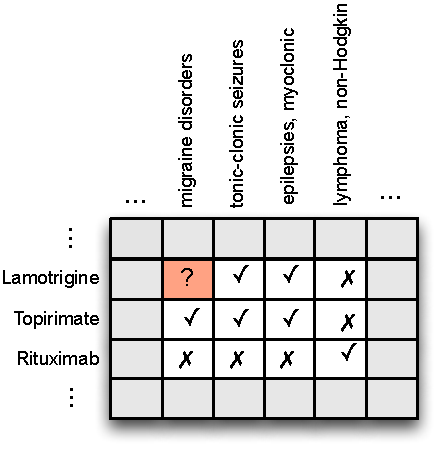
\includegraphics[width=0.6\linewidth]{ch2-figures/Figure4.pdf}
  \end{center}
  \caption[Using prior knowledge to calculate drug-drug and
    indication-indication similarity]{Using prior knowledge to
    calculate drug-drug and indication-indication similarity.  We
    represent known usage as a matrix where row i represents drug i
    and column j represents indication j.  A check in entry (i,j)
    indicates that the drug i is used to treat the indication j, while
    a cross indicates the converse.  We are interested in whether a
    given drug, lamotrigine, is used to treat migraine disorders.  We
    thus ask — how similar is the known usage of lamotrigine to other
    drugs we know are used to treat migraine disorders?  Topirimate is
    used to treat migraine disorders, and lamotrigine is similar to it
    in that both are used to treat tonic-clonic seizures and myoclonic
    epilepsies, but not non-Hodgkin's lymphoma.  This similarity in
    usage profile suggests that it is more likely to be used to treat
    migraine disorders than, say, Rituximab.  We measured this
    similarity using the maximum cosine and Jaccard similarity of
    lamotrigine versus all drugs known to treat the indication.  We
    calculate the similarity between indications based on known usage
    using the same data, with the roles of drugs and indications
    reversed.}
  \label{fig:short}
\end{figure}

The DrugBank 3.0 \cite{Knox2011} database provides information on
6,711 drugs and their molecular targets, pathways, and indications.
The annotator was used to map DrugBank drug names and indications to
our target sets of drugs and indications. Molecular targets, pathways,
and drug categories were also extracted for each drug.  We calculated
similarity features analogous to the Medi-Span similarity features,
along with other features that capture similarity with respect to
molecular targets, pathways, and drug categories.  As with the
Medi-Span derived features, we removed test usages from DrugBank
before calculating features.  

\subsection{Training a predictive model}
The gold standard dataset was randomly split into 35,050 training and
8,784 test examples.  We trained an SVM classifier using radial basis
function kernels on the training examples using the e1071 library in
R.  The performance of the classifier was tested on the test examples.
We also trained and tested classifiers using subsets of the features
to assess the contribution of different groups of features.  We then
trained a classifier on the entire gold standard and applied it to all
2,362,950 possible drug-indication pairs.  In all cases, we used
ten-fold cross validation on the training data and the “1-se” rule to
select the cost hyperparameter for the SVM models.  Estimates of each
prediction’s class membership probabilities were obtained via logistic
regression \cite{Platt1999}.  We used a probability threshold of 0.99
in order to limit the set of predicted usages to the most confident
predictions.  This hard threshold was not tuned in any way; thus our
final set of predicted novel off-label usages could possibly be
improved by adjusting this threshold.  However, this is a very simple
way to restrict our attention to the most confident predictions.

\subsection{Identifying known usages}
Known usage was determined by presence in Medi-Span or the NDF-RT –
drug-indication pairs absent from both are assumed to be novel usages.
Review of these usages revealed that indications were sometimes
closely related to known usages — e.g., glaucoma and open angle
glaucoma.  We addressed this problem using biomedical ontologies,
which organize biomedical concepts into hierarchies — e.g., amok is a
subtype of the parent concept mania.  Specifically, we removed
predicted usages in which the indication is a subtype of a known usage
indication in SNOMED-CT, or is the direct parent of a known usage
indication in SNOMED-CT.  As a final check against Medi-Span and
NDF-RT, we manually reviewed predicted usages remaining after
validation in FAERS, MEDLINE and SIDER2 (described below), removing 63
usages that were not detected as known usages by the methods described
above.

\subsection{Validation by FAERS, MEDLINE and mechanistic plausibility}
FAERS case reports contain explicit used-to-treat links between drugs
and indications.  We validated predicted usages using these links
using public domain case reports from Q3 2007 through Q2 2012.  FAERS
drugs and indications were mapped to UMLS CUI’s, yielding a set of 3
million drug-indication reports covering 160,989 unique pairs.  Only
3,756 out of 8,861 (43\%) positive examples of drug usages in our gold
standard dataset appear at least once in FAERS.  We required at least
10 such reports because this threshold results in a false positive
rate of less than 0.005 when applied to the gold standard dataset.

MEDLINE entries are manually annotated with MeSH terms, Supplementary
Concepts for drugs, and subheadings that provide further context for
the annotation.  For instance, an article about treatment of wet
macular degeneration by bevacizumab would be annotated with “wet
macular degeneration/drug therapy*” and, separately, “bevacizumab.”
We downloaded the complete set of annotations for MEDLINE entries from
2002-2012.  MeSH annotations were filtered for indications with the
drug therapy sub-heading and mapped to UMLS CUI’s using the NCBO
Annotator.  The Substance annotations were also mapped to UMLS CUI’s
using the Annotator.  If no MeSH term corresponded exactly to the
indication, we expanded the indication to the more general MeSH term,
e.g., ‘malignant neoplasm of the ovary’ was interpreted as ‘ovarian
neoplasm’.  As in Avillach et al \cite{Avillach2013}, we considered
usages with at least three articles annotated with both the indication
and the drug to be well-supported by MEDLINE.

We assessed the mechanistic plausibility of predicted usages by
examining patterns of gene expression induced by the drug and
indication.  Briefly, we performed gene set enrichment analysis on
gene expression data from the NCBI Gene Expression Omnibus (GEO)
\cite{Edgar2002} and the Connectivity Map \cite{Lamb2006} to identify
biological pathways and expression modules that are inversely
regulated between pairs of diseases and drugs, suggesting a possible
basis for a therapeutic association \cite{Sirota2011}.  

\subsection{Removal of drug adverse events}
We used drug adverse events listed in the SIDER 2 resource to minimize
the impact of confounding causal relationships on our results.  67 out
of 406 novel, well-supported off-label usages matched SIDER 2 entries.
However, manual review of these matches revealed that only 28
drug-indication pairs were likely to be bona fide drug related adverse
events.  This is due to the fact that SIDER 2 is not curated and thus
includes many spurious results such as indications being listed as
adverse events.  After removal of the true adverse events, 403
off-label usages remained.  Calculation of risk and cost indices The
cost and risk indices are motivated by the observation that off-label
usages do not all have the same urgency for further investigation.
Decision analysis suggests that we rank usages based on their expected
utility — i.e., the desirability of possible outcomes of the use,
weighted by the probability each outcome \cite{Meltzer2011}.  For
example, the use of a cheap antibiotic with few side effects to treat
a rare condition has a lower urgency for follow-up than the use of an
expensive drug, with severe side effects, to treat a common disorder.
We approximated this approach by developing quantitative indices of
drug cost and risk associated with drug usage based on known adverse
events

The cost index was calculated by ranking drugs by their mean unit cost
in Medi-Span (a drug may have multiple unit costs due to different
formulations, etc.).  The ranks were normalized to lie between 0 and
1, with the most expensive drug having a score of 1.  The risk index
for each drug was based on an estimate of the expected disutility of
adverse events associated with using that drug in Medi-Span. Briefly,
we assigned quantitative disutility values to adverse events
associated with drugs in Medi-Span.  The expected disutility of drug
use due to adverse events was then estimated as the weighted sum of
the disutilities for associated adverse events, with the weights given
by probabilities estimated from Medi-Span’s estimates of the frequency
of the adverse events.  Drugs were ranked by expected disutility and
the ranks normalized to lie between 0 and 1 such that the riskiest
drug had a value of 1. The lower and upper quartiles of the cost and
risk index values observed in the 403 well-supported novel usages were
used as thresholds for defining high and low risk or cost groups.

\section{Results}
We trained an SVM classifier to recognize used-to-treat relationships
between drugs and indications and applied the classifier to all
possible drug-indication pairs.  Filtering for high prediction
confidence yielded 14,174 high confidence used-to-treat
relationships. We then removed known usages listed in two curated
sources of known usage — Medi-Span and the National Drug File –
Reference Terminology (NDF-RT) \cite{Brown2004}, leaving 6,142
predictions that could be novel off-label usages.  We assessed support
for the putative novel off-label uses in independent and complementary
data sources including the FDA’s Adverse Event Reporting System
(FAERS) and MEDLINE.  When possible, we also assessed the biological
plausibility of these usages using publically available gene
expression data \cite{Sirota2011}.  We reduce spurious results arising
from drug adverse events by filtering these usages using SIDER 2,
yielding a final set of 403 well-supported novel off-label
usages. Overall, we tested 1,602 unique drugs and 1,475 unique
indications, resulting in 403 well-supported novel off-label usages
that we prioritized by their potential risks and cost.

\subsection{A classifier for detecting used-to-treat relationships}
Classifiers such as support vector machines map inputs, or features,
to outputs.  In this study, the inputs come from clinical text and
domain knowledge about drugs from Medi-Span and DrugBank.  Medi-Span
encodes information about know usages, while Drugbank encodes
information about drug targets and mechanisms of action.  For each
drug–indication pair, we construct a set of features that the
classifier uses to predict whether a used-to-treat relationship holds
between the drug and indication.  The classifier learns to make
accurate predictions using inputs for which we know the desired
output, i.e., positive or negative examples of known usages
\cite{Hastie2009}.  We constructed such a gold standard dataset of
known usages from the Medi-Span Drug Indications Database (Wolters
Kluwer Health, Indianapolis, IN) as positive examples, along with
negative examples constructed as detailed in Methods.  An SVM
classifier was trained on a random subset (80\%) of the gold standard
and achieved a positive predictive value of 0.963, specificity of
0.991, sensitivity of 0.764 and F1 score of 0.852 on the remaining
20\% of the gold standard (see Figure 2.3).  Feature ablation
experiments showed that each group of features contributed to overall
performance, particularly with respect to sensitivity and positive
predictive value (Table 2.1).  Individually, the features learned from
clinical notes in the Stanford Translational Research Integrated Data
Environment (STRIDE) and Medi-Span yielded sensitivities of 0.681 and
0.662 respectively, while all features together resulted in a
sensitivity of 0.764.  In identifying population level associations,
drugs and diseases may also get associated because of causal
relationships (i.e., the drug is causing the disease, as an adverse
drug event) or indirect relationships (i.e., the disease is a common
co-morbidity of an approved indication) rather than used-to-treat
relationships.  We count co-mentions of drugs and indications taking
known indications into account, and as a result, obtain substantially
better performance than previous methods that ignore known indications
\cite{Jung2013}.  Similarly, the PPV achieved using all features was
0.963, substantially better than the 0.936 achieved using only
features derived from just STRIDE and consistent with the hypothesis
that prior knowledge is able to reduce spurious results arising from
causal and indirect relationships \cite{Li2011}.

\begin{table}
\begin{center}
\begin{tabular}{|c|c|c|c|c||}
  \hline Feature set & PPV & Specificity & Recall & F1 \\ \hline\hline
  Naive STRIDE only & 0.771 & 0.964 & 0.483 & 0.594 \\ STRIDE only &
  0.936 & 0.988 & 0.681 & 0.788 \\ Medi-Span only & 0.945 & 0.990 &
  0.692 & 0.778 \\ Drugbank only & 0.831 & 0.981 & 0.377 & 0.518
  \\ STRIDE + Medi-Span & 0.967 & 0.994 & 0.744 & 0.841 \\ STRIDE +
  Drugbank & 0.936 & 0.988 & 0.697 & 0.799 \\ All & 0.963 & 0.993 &
  0.764 & 0.852 \\ \hline
\end{tabular}
\end{center}
\caption[Performance of used-to-treat classifier]{Performance of
  classifier on hold-out test set using different feature sets.  We
  performed feature ablation experiments to assess the contribution of
  different feature sets to the performance of the classifier for
  detecting used-to-treat relationships.  The first column indicates
  the features used to train and test the classifiers.  Classifier
  performance was evaluated in a hold out test set of 1,749 positive
  and 7,035 negative examples of drug usage after training in a set of
  7,112 positive and 27,938 negative examples.  The first row shows
  performance using STRIDE derived features in which co-mentions are
  counted without regard to present known indications in the clinical
  record.}
\end{table}


\begin{figure}
  \begin{center}
    \includegraphics[width=0.9\linewidth]{ch2-figures/Figure2.pdf}
  \end{center}
  \caption[Training a classifier to recognize used-to-treat
    relationships]{Training and testing a classifier to recognize
    used-to-treat relationships.  We created a gold standard of
    positive and negative examples of known drug usage.  Positive
    examples were taken from Medi-Span.  We created negative examples
    by randomly selecting positive examples and then randomly choosing
    a drug and indication with roughly the same frequency of mentions
    in STRIDE as the real usage.  These were then checked against
    Medi-Span to filter out inadvertently generated known usages.  The
    gold standard dataset contained 4 negative examples for each
    positive case.  For each drug-indication pair in the gold
    standard, we calculated features summarizing the pattern of
    mentions of the drugs and indications in 9.5 million clinical
    notes from STRIDE. We used Medi-Span and Drugbank to calculate
    features summarizing domain knowledge about drugs and their
    usages.  80\% of the gold standard was used to train an SVM
    classifier, and the resulting model was tested on the remaining
    20\%.  }
  \label{fig:short}
\end{figure}


\subsection{Predicting novel off-label usages}
We applied an SVM trained on the entire gold standard dataset to all
2,362,950 possible drug-disease pairs to find used-to-treat
relationships.  SVMs do not output class membership probabilities;
thus we fit a logistic regression model to the output of the SVM to
estimate the probability of the used-to-treat relationship being true
for a given drug-disease pair \cite{Platt1999}.  Applying a cut-off of
0.99 to this estimate yielded 14,174 high confidence used-to-treat
relationships, which we interpret as potential drug-indication usage
pairs.  After filtering out known usages listed in Medi-Span and the
National Drug File – Reference Terminology (NDF-RT) \cite{Brown2004},
we removed usages in which the predicted indication is closely related
to already known indications as described in Methods, resulting in
6,142 high confidence novel usages.  Because approved usages are
presumably known, these are interpreted to be high confidence novel
off-label usages.

\subsection{Support in FAERS, MEDLINE and SIDER 2}
The 6,142 high confidence novel off-label usages were examined for
positive support in two independent and complementary data sources
(FAERS and MEDLINE) and for negative support in SIDER 2 as described
in Methods.  FAERS case reports explicitly link indications and the
drugs used to treat them \cite{WeissSmith2011}.  These reports are
created by patients, health care providers and drug manufacturers, and
directly reflect clinical practice.  In contrast, MEDLINE provides
curated annotations of the biomedical literature with terms from the
National Library of Medicine’s Medical Subject Headings (MeSH)
vocabulary.  We found that 766 novel off-label usages are supported by
at least 10 records in FAERS, and 537 of those are also supported by
at least two articles co-annotated with the drug and indication in
MEDLINE \cite{Avillach2013}.  We then filtered out usages that
appeared to be bona fide drug adverse events listed in SIDER 2 in
order to eliminate drug-disease pairs that are actually drug-adverse
event relationships, leaving us with 466 candidate novel off-label
usages.  We manually examined these to filter out known usages that
were missed in Medi-Span and the NDF-RT, leaving us with 403
well-supported novel off-label usages.

These usages cover 210 drugs and 184 indications, and recapitulate
previously noted patterns of off-label usage (Figure 2.4).  Medical
specialties such as oncology have been noted to have high rates of
off-label usage \cite{Poole2004}. Consistent with this observation,
there are many cancer drugs among our results — e.g., ofatumumab for
non-Hodgkin’s lymphoma \cite{Hagenbeek2008} and fludarabine for
chronic myelogenous leukemia \cite{Or2003}.  Other previously noted
usage patterns include the use of the anti-seizure medications such as
pregabalin and lamotrigine for migraines
\cite{Lampl2005,Pizzolato2011}, and the use of immuno-modulators such
as etanercept and adalimumab, two Tumor Necrosis Factor (TNF)
inhibitors, for systemic lupus erythematosus (SLE)
\cite{Merrill2010,Merrill2010b}.  Interestingly, etanercept and
infliximab, another TNF inhibitor, have both been investigated as
treatments for SLE \cite{Hayat2007}, lending support to the
classifier’s prediction.  However, etanercept and adalimumab have also
been implicated in causing SLE \cite{Shakoor2002,Martin2011}.  Thus,
in this case both the used-to-treat and causal relationships may be
true.

\begin{figure}
  \begin{center}
    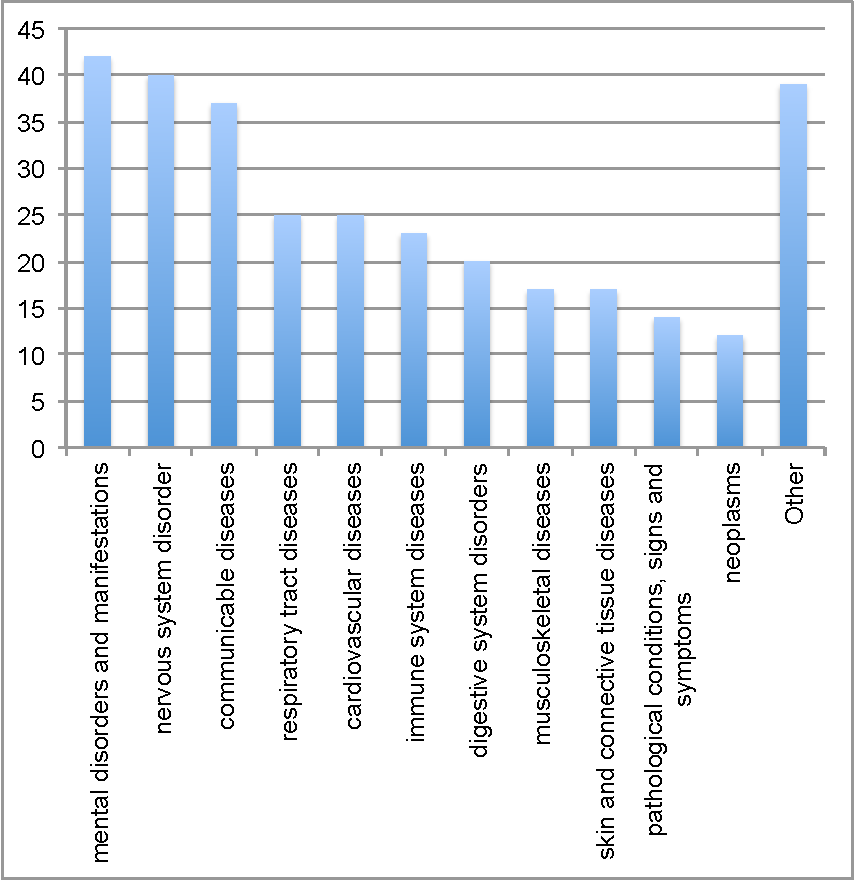
\includegraphics[width=0.9\linewidth]{ch2-figures/Figure3.pdf}
  \end{center}
  \caption[Distribution of indication classes in predicted novel
    usages]{Distribution of indication classes in predicted novel
    usages.  Each indication for the 403 high confidence novel usages
    with support in FAERS and MEDLINE was mapped to the first level of
    the NDF-RT disease hierarchy.  63 usages were not mapped to NDF-RT
    and were left out of this chart.  }
  \label{fig:short}
\end{figure}


\subsection{Plausibility based on mechanisms of action}
We also evaluated the plausibility of the novel, predicted off-label
usages using previously published methods \cite{Sirota2011} applied to
gene expression data from the Connectivity Map \cite{Lamb2006} and
NCBI Gene Expression Omnibus \cite{Edgar2002}.  Briefly, if a drug
modulates gene expression in the opposite manner than a disease
condition, the drug is considered a plausible treatment for the
indication.  This approach requires gene expression data for both drug
exposure and the disease condition.  Of our well-supported novel
usages, two had appropriate publically available data and both yielded
significant gene sets suggesting possible mechanisms of action.  Given
sparse coverage of drugs and diseases in public data, it is difficult
to apply this process systematically.  Nevertheless, this method
yielded testable hypotheses regarding mechanisms of action.  For
instance, simvastatin is linked to diabetes by PPAR-gamma; simvastatin
treatment enriches a gene set known to be activated by PPAR-gamma
activity, while PPAR-gamma agonists, e.g., thiazolinediones, are known
to be used to treat diabetes \cite{Grip2002,Altshuler2000}.

\subsection{Manual validation of the predicted usages}
Examination of the 403 well-supported novel off-label usages revealed
terminological challenges.  For instance, we predict that alendronic
acid is used to treat osteopenia, the clinical precursor to
osteoporosis.  However, Medi-Span and the NDF-RT list the indication
as osteoporosis instead of osteopenia — i.e., they encode the
used-to-prevent relationship. Such issues reflect challenges in
normalizing medical terms.  As a result, although we can detect
used-to-treat relationships quite well, recognizing whether or not
uses are already known is difficult.

Some predicted uses represent bona fide new uses confirmed in the
biomedical literature by case reports, clinical trials, or resources
such as MedlinePlus, but not yet incorporated in our curated sources
of known usage (see Table 2.2 for selected examples).  For instance,
our system predicts that bevacizumab is used to treat ovarian cancer.
This usage has been shown to improve progression free survival in a
phase III trial \cite{Perren2011} and has been approved in the EU, but
does not yet appear in Medi-Span, Drugbank, the NDF-RT or MedlinePlus.
These results show that it is possible to detect emerging off-label
use before it has been officially recognized.


\begin{table}
\begin{center}
\begin{tabular}{|c|c|c|c||}
  \hline Drug Name & Event Name & FAERS & MEDLINE \\ & & Support &
  Support \\ \hline\hline Simvastatin & diabetes mellitus & 1369 & 33
  \\ Tacrolimus & rheumatoid arthritis & 404 & 45 \\ Pregabalin &
  migraine disorders & 152 & 3 \\ Etanercept & lupus erythematosus,
  systemic & 79 & 5 \\ Lamotrigine & migraine disorders & 75 & 6
  \\ Adalimumab & lupus erythematosus, systemic & 71 & 3 \\ Rituximab
  & hodgkin disease & 51 & 48 \\ Daptomycin & osteomyelitis & 45 & 20
  \\ Fludarabine & waldenstrom macroglobulinemia & 39 & 66
  \\ Infliximab & pyoderma gangrenosum & 34 & 68 \\ Erlotinib &
  malignant neoplasm of ovary & 28 & 16 \\ \hline
\end{tabular}
\end{center}
\caption[Selected predicted novel off-label usages]{Selected predicted
  novel off-label usages.  Predicted, novel drug usages with
  substantial support in FAERS.  FAERS Support for each
  drug-indication pair is the number of distinct case reports in FAERS
  in which the drug was explicitly listed as being used to treat the
  indication.  }
\end{table}


\subsection{Prioritizing predicted off-label usages for further investigation}
We designed indices of drug risk and cost using adverse event
associations and unit cost data from Medi-Span to objectively triage
usages for further investigation. The drug risk index is normalized to
lie between 0 and 1, with a value of 0 for drugs with no adverse event
associations in Medi-Span (811 out of 1,602 drugs) and 1 for drugs
associated with many serious adverse events.  Not surprisingly, drugs
with the highest risk indices were immunosupressants, such as
mycophenalate mofetil, and anti-tumor agents, such as gemtuzumab,
clofarabine, bevacizumab, and fludarabine.  Well-supported novel
off-label usages had risk indices ranging from 0.002 for amphotericin
to a maximum of 0.995 for clofarabine.

The drug cost index is based on the mean unit price for the drug in
Medi-Span and is also normalized to lie between 0 and 1, with a value
of 1 for the drug with the highest mean unit cost in Medi-Span.  The
unit cost is an imperfect measure of actual treatment cost — for
instance, it may be for a quantity that is sufficient for multiple
treatments.  Nevertheless, the cost index provides a partial ordering
that is useful for relative ranking because the drugs with the highest
cost index are expensive, targeted therapies such as ranibizumab,
while the drugs with low cost index values are over the counter agents
such as magnesium chloride and iodine.

We used the risk and cost indices to group well-supported novel
off-label usages into high risk, high cost and low risk, low cost
usages, resulting in 28 and 51 usages, respectively (the top 5 usages
in each group are listed in Table 2.3).  We defined thresholds for highs and
lows by looking at the distribution of the risk and cost indices for
the 403 well-supported usages and choosing the upper and lower
quartiles as cutoffs. For example, the upper quartile for the 403
well-supported usages had risk index value 0.828, which defines the
threshold for the high-risk group. For the 403 well-supported usages,
\textbf{Figure 2.1} shows the high–high (28 drug-indication pairs) and
low–low groups (51 drug-indication pairs). Many (16 of 28) of the high
risk, high cost usages involved anti-tumor agents being used to treat
unapproved tumor types. In contrast, the low cost, low risk usages
contain many over the counter drugs such as vitamin E, as would be
expected.

\begin{table}
\begin{center}
\begin{tabular}{|l|l|c|c|c|c||}
  \hline Drug Name & Indication & FAERS & MEDLINE & Risk & Cost \\ & &
  Support & Support & Index & Index \\ \hline\hline
  \multicolumn{6}{|l|}{High risk, high cost usages} \\ \hline
  Docetaxel & Malignant neoplasm & 604 & 640 & 0.964 & 0.949\\ & of
  prostate & & & & \\ \hline Clofarabine & Leukemia, myelocytic,& 341
  & 37 & 0.995 & 0.869 \\ & acute & & & & \\ \hline Rituximab &
  Purpura, & 259 & 169 & 0.940 & 0.821 \\ & thrombocytopenic, & & & &
  \\ & idiopathic & & & & \\ \hline Bevacizumab & Malignant neoplasm &
  170 & 89 & 0.991 & 0.879 \\ & of ovary & & & & \\ \hline Paclitaxel
  & Malignant neoplasm & 122 & 421 & 0.956 & 0.776 \\ & of stomach & &
  & & \\ \\ \hline \multicolumn{6}{|l|}{Low risk, low cost usages}
  \\ \hline Folic acid & mental depression & 493 & 18 & 0.082 & 0.102
  \\ \hline Methadone & depressive disorder & 162 & 33 & 0.002 & 0.167
  \\ \hline Folic acid & hyperlipidemia & 138 & 10 & 0.082 & 0.102
  \\ \hline Megestrol & carcinoma, non-small & 79 & 4 & 0.002 & 0.238
  \\ & cell lung & & & & \\ \hline Folic acid & diarrhea & 67 & 10 &
  0.082 & 0.102 \\ \hline
\end{tabular}
\end{center}
\caption[Ten validated Drug-AEs]{List of ten validated Drug-AEs and
  their support in FAERS as well as MEDLINE}
\end{table}


\section{Discussion}
Off-label usage of drugs is an important enough aspect of drug safety
to warrant a full issue (May 2012) of Nature Clinical Therapeutics and
Pharmacology devoted to the topic \cite{Epstein2012}.  Currently the
most comprehensive information about off-label drug usage is from the
National Disease and Therapeutic Index (IMS Health, Plymouth Meeting,
PA), which relies on periodic surveys of office-based physicians. We
believe that off-label use can be learned systematically, in a
data-driven manner directly from electronic medical records.  Our work
represents the first effort to detect novel off-label usage from
clinical free text over the entire range of drugs and indications
observed in the medical record.  We also developed quantitative risk
and cost indices as a way to prioritize the novel usages for further
investigation.

In the past, NLP has been applied to the problem of detecting
used-to-treat relationships between drugs and indications in clinical
text.  State of the art NLP approaches require training text in which
drug and indication mentions are labeled, along with the relationships
between them.  In contrast, association based approaches that use
counts of drug and indication mentions are more scalable, but limited
by confounding causal and indirect relationships.  We have developed
an automated method for detecting novel off-label usages from clinical
text that does not require training text and addresses confounding
relationships by incorporating prior knowledge about drug usage.  We
applied this method to 1,602 drugs and 1,475 indications to identify
6,142 novel off-label usages, 403 of which are well supported by
evidence in independent and complementary datasets.

Our methods have important limitations.  First, our work focuses on
one form of off-label use — the use of drugs to treat unapproved
indications — and does not detect off-label use with respect to age,
gender, dosage and contraindications.  Second, co-morbidities and drug
adverse events may still lead to spurious used-to-treat relationships
despite our efforts to reduce their impact on our results. Third,
although our method can detect used-to-treat relationships between
drugs and indications with high specificity and good sensitivity, the
task of recognizing whether the knowledge is already known is more
difficult than might be expected.  This difficulty was not due to
errors in recognizing terms in clinical text but rather due to
mismatches in the language used to describe indications in Medi-Span
and the NDF-RT versus clinical text and FAERS.  A systematic listing
of such indication mismatches could identify areas in ontologies and
terminologies that need improvement — and would be a data-driven way
to identify portions of terminologies for review.  Fourth, the risk
and cost indices have some shortcomings.  For instance, the cost index
ignores the fact that dosage and duration of treatment for off-label
usages may differ from approved uses, and our risk index does not take
the dependence of adverse events on dosage, co-morbidities, and
poly-pharmacy into account.  Finally, in this work we have aimed to
produce a list of highly confident predictions of novel off-label
usages so we require corroboration of predictions in FAERS, which has
much lower recall in the test set than the classifier.  Thus the
overall method sacrifices sensitivity for greater specificity.  This
is appropriate for our aim in this work, but other studies may require
a different trade off between sensitivity and specificity.  For
instance, if we were concerned exclusively with potentially risky
usages, we might not require support in FAERS and instead filter for
usages involving drugs associated with known serious side effects that
don’t always get reported.  We note that our method can be modified
for such use cases.

These limitations notwithstanding, our study is the first large-scale
characterization of off-label usage using fully automated methods to
combine information from clinical notes with prior knowledge and to
provide a ranking of the learned usages on risk and cost.  It is a
step towards systematic, data-driven monitoring of off-label usage.
The method has characteristics that allow it to generalize to sites
beyond Stanford.  First, the system does not require training text
labeled with mentions of drugs and indications, and the relationships
between them.  Second, our method is very flexible with respect to the
target drug and indication vocabulary.  Third, the system is very fast
— annotation of 9.5 million clinical notes takes only two hours on a
single machine; constructing features, training a classifier and
making predictions takes an additional few hours.  It is thus
conceivable to process clinical text from a large number of sites,
providing a picture of off-label usage across a wide spectrum of
institutions.

Most importantly, our method was able to detect usages that were
documented in the biomedical literature, and in one case approved in
the EU, despite not appearing in any of our curated sources of known
usage.  This suggests that such systems could potentially provide an
automated learning system for off-label usage.  Such as system could
flag emerging usages before they come to the attention of the broader
medical community, regulatory agencies and drug manufacturers, in much
the same way that Google Flu Trends can provide an early warning of
flu trends in advance of CDC data \cite{Ginsberg2009}.  We speculate
that applying our method to a wider range of clinical text from
multiple sites can provide a timelier and more comprehensive picture
of off-label usage than is currently possible
\cite{Halevy2009,Banko2001}.

